\documentclass{article}
\usepackage[utf8]{inputenc}

\usepackage{graphicx}
\graphicspath{{./images/}}

\usepackage{amsmath}
%\usepackage{amssymb}
%\usepackage{mathtools}

\providecommand{\norm}[1]{{\lVert#1\rVert}}

\usepackage{geometry}
\geometry{left=1.5cm, right=1.5cm, top=1.5cm, bottom=1.5cm}

\title{Formulaire de Physique I - Mécanique}
\author{C.B.}
\date{Semestre d'automne 2019}

\begin{document}
\maketitle
\section{Notions mathématiques}
\subsection{Produit scalaire et produit vectoriel}
\begin{align}
	&\norm{\vec a \wedge \vec b} = \norm{\vec a} \cdot \norm{\vec b} \cdot \sin(\theta)
	&\norm{\vec a \cdot \vec b} = \norm{\vec a} \cdot \norm{\vec b} \cdot \cos(\theta)
\intertext{En particulier:}
	&\vec a \wedge \vec b \perp \Pi(\vec a, \vec b)
	&\vec a \perp \vec b \iff \vec a \cdot \vec b = 0 \\
\intertext{Produit mixte et double produit vectoriel:}
	&\begin{cases}
		(\vec a \wedge \vec b) \cdot \vec c = (\vec c \wedge \vec a) \cdot \vec b \\
		(\vec a \wedge \vec b)\cdot \vec c = 0 \iff \vec a, \vec b, \vec c \text{ coplanaires}
	\end{cases}
	&\vec a \wedge (\vec b \wedge \vec c) = (\vec a \cdot \vec c)\vec b - (\vec a \cdot \vec b)\vec c
\end{align}

\subsection{Systèmes de coordonnées}
\subsubsection{Système de coordonnées cylindriques}
Position projetée sur les axes:
\begin{equation}
	\vec r = \rho \hat e_\rho + z \hat e_z
\end{equation}
Vitesse projetée sur les axes:
\begin{equation}
	\vec v = \dot{\vec{r}} = \dot \rho \hat e_\rho + \rho \dot \phi \hat e_\phi + \dot z \hat e_z
\end{equation}
Accélération projetée sur les axes:
\begin{equation}
	\begin{cases}
		a_\rho = \ddot \rho - \rho \dot \phi^2 \\
		a_\phi = \rho \ddot \phi + 2 \dot \rho \dot \phi \\
		a_z = \ddot z 
	\end{cases}
\end{equation}

\subsubsection{Système de coordonnées sphériques}
Position projetée sur les axes:
\begin{equation}
	\vec r = r \hat e_r
\end{equation}
Vitesse projetée sur les axes:
\begin{equation}
	\vec v = \dot{\vec r} = \dot r \hat e_r + r \dot \theta \hat e_\theta + r \dot \phi \sin(\theta) \hat e_\phi
\end{equation}
Accélération projetée sur les axes:
\begin{equation}
	\begin{cases}
	a_r 		= \ddot r - r \dot \theta^2 - r \dot \phi^2 \sin^2(\theta) \\
	a_\theta	= r \ddot \theta + 2 \dot r \dot \theta - r \dot \phi^2 \cos(\theta)\sin(\theta) \\
	a_\phi		= r \ddot \phi \sin(\theta) + 2r \dot \phi \dot \theta \cos(\theta) + 2 \dot r \dot \phi \sin(\theta)
	\end{cases}
\end{equation}

\section{Mécanique du point}
\subsection{Les 3 lois de Newton}
\subsubsection{Loi d'inertie}
\begin{center}
	\emph{``Tout corps persévère dans l'état de repos ou de mouvement uniforme en ligne droite, \\
	 à moins qu'une force n'agisse sur lui et ne le contraigne à changer d'état.''}
\end{center}
\begin{equation}
	\boxed{\vec F = \vec 0 \Leftrightarrow \text{MRU}}
\end{equation}
(MRU = Mouvement Rectiligne Uniforme)

\subsubsection{Principe fondamental de la dynamique (\textit{Lex Secunda})}
\begin{center}
	\emph{``Les changements dans le mouvement d'un corps \\ sont proportionnels à la force et se font dans la direction de la force.''}
\end{center}
\begin{equation} \label{eq:lexsecunda}
	\boxed{\vec F = m \vec a}
\end{equation}
On a aussi la formule plus universelle, qui prend en compte les éventuels changements de masse du système (et qui est donc équivalente à la première dans les systèmes sans changement de masse):
\begin{equation} \label{eq:lexsecundap}
	\vec F = \dot{\vec p}
\end{equation}

\subsubsection{Loi d'action-réaction}
\begin{center}
	\emph{``A chaque action, il y a toujours une réaction égale et opposée;\\
	si un corps exerce une force sur un autre,\\
	cet autre corps exerce une force égale et opposée sur le premier.''}
\end{center}
\begin{equation}
	\boxed{\vec F_{1 \to 2} = - \vec F_{2 \to 1}}
\end{equation}

\subsection{Oscillateur harmonique}
\subsubsection{Loi de Hooke}
Force exercée par un ressort:
\begin{equation}
	\boxed{\vec F = -k \Delta x}
\end{equation}
où $\Delta x$ est la différence entre la position au repos de l'extrémité du ressort et la position actuelle de l'extrémité ressort (peut être positive ou négative).

\subsubsection{Équation du mouvement d'un oscillateur harmonique}
L'équation du mouvement d'un oscillateur harmonique est de la forme
\begin{equation}
	m \ddot x = -\omega_0^2 x
\end{equation}
où on nomme $\omega_0$ la vitesse angulaire du mouvement. Cette équation différentielle admet deux formes de solution:
\begin{align}
	&x(t) = A\cos(\omega_0 t) + B\sin(\omega_0 t)\\
	&x(t) = C\sin(\omega_0 t + \phi)
\intertext{Comme $\sin(\theta + \pi/2) = \cos(\theta)$, on peut également avoir
}
	&x(t) = D\cos(\omega_0 t + \phi')
\end{align}

\section{Énergie et travail}
\subsection{Forces de frottement}
Une force de frottement s'oppose toujours au mouvement d'un corps.

\subsubsection{Frottement sec statique}
L'aspect important de la force de frottement sec statique n'est pas sa valeur, mais sa norme maximale:
\begin{equation}
	\boxed{\norm{\vec F_s} \leq \mu_s \cdot \norm{\vec N}.}
\end{equation}
La force de frottement sec statique s'oppose exactement aux forces qui tentent de déplacer l'objet le long de la surface de contact, de telle façon à ce que l'objet reste statique (somme des forces $= \vec 0 \iff$ pas de changement de vitesse):
\begin{equation}
	\vec F_s = -\vec F_{\parallel}
\end{equation}
Une fois sa norme maximale dépassée, la force de frottement sec statique ne peut plus équilibrer les autres forces parallèles à la surface de contact, et l'objet se met à bouger.

\subsubsection{Frottement sec cinétique}
La force de frottement cinétique est de sens opposé à la vitesse du corps.
\begin{equation}
	\boxed{\vec F_c = -(\mu_c \cdot \norm{\vec N})\hat v}
\end{equation}

\subsection{Quantité de mouvement et impulsion}
\subsubsection{Quantité de mouvement}
On définit la \textbf{quantité de mouvement} d'un point matériel par
\begin{equation}
	\boxed{\vec p = m \vec v.}
\end{equation}
La seconde loi de Newton \eqref{eq:lexsecundap} dit que la quantité de mouvement d'un point matériel ne change pas tant que la somme des forces extérieures est nulle (et que la masse ne change pas).

\subsubsection{Impulsion}
On définit l'\textbf{impulsion} d'une force $\vec F$ appliquée sur un point matériel entre un instant 1 et un instant 2 par
\begin{equation}
	\vec I_{12} = \int_1^2 \vec F \cdot dt.
\end{equation}
Si $\vec F$ est la résultante des forces s'appliquant sur le point matériel, alors $\vec F = m \vec a$ et cette équation se simplifie en
\begin{equation}
	\boxed{\vec I_{12} = \vec p_2 - \vec p_1.}
\end{equation}

\subsection{Énergie cinétique, travail et puissance d'une force}
\subsubsection{Énergie cinétique}
On définit  l'\textbf{énergie cinétique} d'un point matériel par
\begin{equation}
	\boxed{K = \frac12 m \norm{\vec v}^2}
\end{equation}

\subsubsection{Travail d'une force}
On définit le \textbf{travail} d'une force $\vec F$ appliquée sur un point matériel entre un point 1 et un point 2 par
\begin{equation} \label{eq:def_travail}
	W_{12} = \int_1^2 \vec F \cdot d \vec r.
\end{equation}
Si la trajectoire entre le point 1 et le point 2 est rectiligne et la force reste constante sur cette trajectoire, cette équation se simplifie en
\begin{equation}
	\boxed{W_{12} = \norm{\vec F} \cdot d_{12}}
\end{equation}
où $d_{12}$ est la distance entre le point 1 et le point 2.\\
Si $\vec F$ est la résultante des forces s'appliquant sur le point matériel, alors $\vec F = m \vec a$ et l'intégrale \eqref{eq:def_travail} se simplifie en
\begin{equation} \label{eq:travail-K}
	W_{12} = K_2 - K_1
\end{equation}

\subsubsection{Puissance d'une force}
On définit la \textbf{puissance instantanée} d'une force par
\begin{equation}
	P = \frac{dW}{dt}.
\end{equation}
Or
\begin{equation}
	\frac{dW}{dt} = \frac{\vec F \cdot d \vec r}{dt} = \vec F \cdot \vec v
\end{equation}
(à compléter parce que je sais pas trop comment inscrire ça dans le reste de la théorie)\\

\subsubsection{Théorème de l'énergie cinétique}
(mettre également thm de l'énergie cinétique)

\subsection{Force conservative et énergie mécanique}
\subsubsection{Force conservative et énergie potentielle}
Une force conservative est une force dont la valeur dépend uniquement de la position à laquelle elle est évaluée. Ainsi, on peut introduire la notion du potentiel $V(\vec r)$ d'une force conservative, par lequel la force est déterminée.

\subsection{Énergie mécanique}
Si $\vec F$ est conservative, \eqref{eq:def_travail} donne
\begin{equation}
	W_{12} = \int_1^2 \vec F(\vec r) \cdot d \vec r = V(\vec r_2) - V(\vec r_1).
\end{equation}
On définit l'{énergie mécanique} d'un point matériel comme la somme de son énergie cinétique et de l'énergie potentielle de chacune des forces conservatives par lesquelles il est affecté:
\begin{equation}
	\boxed{E = K + \sum_{\vec F} V_{\vec F}(\vec r).}
\end{equation}
Si toutes les forces qui agissent sur le point matériel sont conservatives, $E$ est une constante.


\subsection{Équilibre et petites oscillations d'un oscillateur harmonique}
L'étude de la fonction $V(x)$ permet de déterminer les points d'équilibre, ainsi que la fréquence des petites oscillations autour des points d'équilibre stable.\\
(à compléter)

\section{Mouvements de rotation}
\subsubsection{Vitesse angulaire}
\begin{equation}
	\omega = \frac{d\phi}{dt}
\end{equation}
Vitesse d'un point $A$ quelconque selon la vitesse angulaire:
\begin{equation}
	\vec v_A = \vec \omega \wedge \vec r_A.
\end{equation}
Si un point est soumis à plusieurs rotations, les vitesses angulaires s'ajoutent:
\begin{equation}
	\vec v_A = \left(\sum \vec \omega \right) \wedge \vec r_A
\end{equation}

\subsubsection{Moment de force}
\begin{equation}
	\boxed{\vec M_O(\vec F) = \vec r \wedge \vec F}
\end{equation}

\subsubsection{Moment cinétique}
\begin{equation}
	\boxed{\vec L_O = \vec r \wedge \vec p}
\end{equation}

\subsubsection{Théorème du moment cinétique}
\begin{equation}
	\boxed{\frac{d \vec L_O}{dt} = \vec M_O}
\end{equation}

\subsubsection{Théorème du transfert}
Le théorème du transfert permet de calculer le moment cinétique en un AAAAAAAAAAAAAAAAAAAAAAAAAAAAAAAAAAAAAAAAAAAAAAAAAAAAAAAAAAAAAAAAa
\begin{equation}
	\vec L_O = \overrightarrow{OA} \wedge m \vec v_A + \vec L_A
\end{equation}

\subsubsection{Moment d'inertie}
AAAAAAAAAAAAAAAAAAAAAAAAAAAAAAAAAAAAAAAAAAAAAAAAAAAAAAAAAAAAAAAAAAAAAAAAAAAAAAAAAAAA

\section{Le solide indéformable}
\subsection{Centre de masse}
On définit la position du \textbf{centre de masse} par
\begin{equation}
	\vec r_G = \frac1M \sum_\alpha m_\alpha \vec r_\alpha
\end{equation}

\subsection{Tenseur d'inertie}
\subsubsection{Par rapport au centre de masse}
Le tenseur d'inertie $\tilde I_G$ d'un solide indéformable par rapport à son centre de masse $G$ est donné par
\begin{equation}
	(\tilde I_G)_{ij} = \sum_\alpha m_\alpha \left[ (\overrightarrow{GP_\alpha})^2 \delta_{ij} - (\overrightarrow{GP_\alpha})_i(\overrightarrow{GP_\alpha})_j \right].
\end{equation}
Les tenseurs d'inertie de quelques solides homogènes communs sont donnés en annexe [REFERENCE?????????????????????????????????????]

\subsubsection{Théorème de Steiner}
Le théorème de Steiner permet de calculer le tenseur d'inertie d'un solide indéformable par rapport à n'importe quel point $A$ du solide, à partir du tenseur par rapport au centre de masse:
\begin{equation}
	(\tilde I_A)_{ij} = (\tilde I_G)_{ij} + M\left[ (\overrightarrow{AG})^2 \delta_{ij} - (\overrightarrow{AG})_i(\overrightarrow{AG})_j \right].
\end{equation}

\subsection{Moment cinétique}
Le moment cinétique d'un solide indéformable est donné par
\begin{equation}
	\vec L_G = \tilde I_G \vec \omega
\end{equation}

%-------------------------------------------------
\pagebreak
\section{Annexe}
\subsection{Tenseurs d'inertie de solides homogènes communs}
Les axes sont choisis ainsi:
\begin{center}
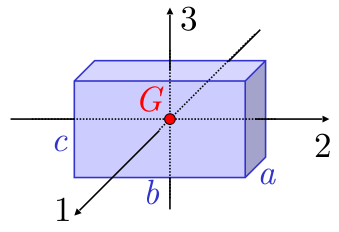
\includegraphics[scale=0.5]{IG_brique} 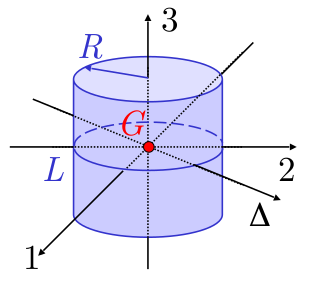
\includegraphics[scale=0.5]{IG_cylindre} 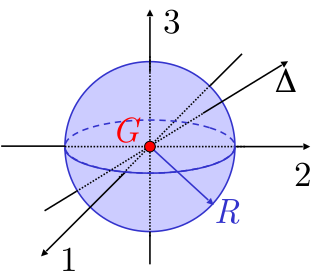
\includegraphics[scale=0.5]{IG_sphere}
\end{center}
On note les composantes des tenseurs diagonaux ainsi:
\begin{equation*}
	\begin{pmatrix}
		I_1 & 0 & 0\\
		0 & I_2 & 0\\
		0 & 0 & I_3
	\end{pmatrix}
\end{equation*}
\allowdisplaybreaks[1]
\begin{align}
\intertext{\textbf{Brique pleine de dimensions $a \times b \times c$}:}
&\tilde{I}_G = \dfrac{m}{12}
\begin{pmatrix}
b^2 + c^2 & 0 & 0 \\
0 & c^2 + a^2 & 0 \\
0 & 0 & a^2 + b^2
\end{pmatrix} \\
\intertext{\textbf{Brique cubique pleine de côté $a$}:}
&\tilde{I}_G = \dfrac{ma^2}{6}
\begin{pmatrix}
1 & 0 & 0 \\
0 & 1 & 0 \\
0 & 0 & 1
\end{pmatrix} \\
\intertext{\textbf{Cylindre plein de rayon $R$ et de longueur $L$}:}
&\tilde I_G = \begin{pmatrix}
	\frac14 mR^2 + \frac{1}{12}mL^2 & 0 & 0\\
	0 & \frac14 mR^2 + \frac{1}{12}mL^2 & 0\\
	0 & 0 & \frac12 mR^2
\end{pmatrix}
\intertext{\textbf{Cylindre vide de rayon $R$ et de longueur $L$}:}
&\tilde I_G = 
\begin{pmatrix}
	\frac12 mR^2 + \frac{1}{12} mL^2 & 0 & 0\\
	0 & \frac12 mR^2 + \frac{1}{12} mL^2 & 0\\
	0 & 0 & mR^2
\end{pmatrix}
\intertext{\textbf{Sphère pleine de rayon $R$}:}
&\tilde I_G = \frac25 mR^2
\begin{pmatrix}
	1 & 0 & 0 \\
	0 & 1 & 0 \\
	0 & 0 & 1
\end{pmatrix}
\intertext{\textbf{Sphère vide de rayon $R$}:}
&\tilde I_G = \frac23 mR^2
\begin{pmatrix}
	1 & 0 & 0 \\
	0 & 1 & 0 \\
	0 & 0 & 1
\end{pmatrix}
\end{align}
\allowdisplaybreaks[0]

\end{document}